\documentclass[11pt]{article}

\usepackage[margin=1.05in]{geometry}
\usepackage{amsmath,amssymb,amsthm}
\usepackage{booktabs}
\usepackage{graphicx}
\usepackage{microtype}
\usepackage{xcolor}
\usepackage{caption}
\usepackage{enumitem}
\usepackage{tikz}
\usetikzlibrary{arrows.meta,positioning,calc,fit,backgrounds}
\usepackage[hidelinks,colorlinks=true,linkcolor={black!70!blue},citecolor={black!70!blue},urlcolor={black!70!blue}]{hyperref}

\definecolor{vblue}{HTML}{2a78d6}
\definecolor{vorange}{HTML}{eb6834}
\definecolor{vaqua}{HTML}{1baf7a}
\definecolor{vink}{HTML}{52514e}

\captionsetup{font=small,labelfont=bf,labelsep=period}

\newtheorem{theorem}{Theorem}
\newtheorem{lemma}[theorem]{Lemma}
\newtheorem{proposition}[theorem]{Proposition}
\newtheorem{corollary}[theorem]{Corollary}
\theoremstyle{definition}
\newtheorem{definition}[theorem]{Definition}
\newtheorem{remark}[theorem]{Remark}
\newtheorem{principle}[theorem]{Design rule}

\newcommand{\Sym}{\mathrm{Sym}}
\newcommand{\sgn}{\mathrm{sgn}}
\newcommand{\Fix}{\mathrm{Fix}}
\newcommand{\ZZ}{\mathbb{Z}}
\newcommand{\Om}{\Omega}
\newcommand{\lean}[1]{{\small\texttt{#1}}}

\title{\bf The Coprime Cascade:\\[2pt]
\large Structural Invariants, Effective Key Length, and Feedback Control\\
in Rotor--Stepping-Switch Cipher Machines}

\author{}
\date{}

\begin{document}
\maketitle
\vspace{-2.2\baselineskip}

\begin{abstract}
\noindent
Electromechanical cipher machines were designed and defended in terms of the
size of their key space, and they were broken in terms of something else. We
give a structural account of what that something else is. We show that each of
the two dominant wartime paradigms carries a proper algebraic invariant of its
reachable permutation set --- a reflector confines every encryption permutation
to the conjugacy class of fixed-point-free involutions, a rotor bank freezes the
signature of its stage permutation, and a split alphabet confines every
permutation to the stabiliser of a partition --- and that these invariants,
not key-space size, are what the classical attacks consumed. We then prove that
even a machine free of all three invariants is broken at the size of its
\emph{state} space rather than its key space, because static key material
composed at the boundary of the cascade is transparent to the statistic that
identifies a trajectory: we prove that the coincidence count of the reduced
stream an attacker forms is independent of the plugboard, and that once a
trajectory is fixed the plugboard is not searched but computed. This settles the
effective key length of a cascade at $\log_2|\Om|$, where $\Om$ is the reachable
state set, and shows the plugboard's $47.1$ bits to be worth zero.

Guided by these two results we specify \emph{Violet}, a cascade of a
reflectorless rotor bank over $\ZZ_{26}$ and a Strowger switch bank over
$\ZZ_{25}$ in which the rotor bank is driven irregularly by the inter-stage tap
through key-set pin rings, while the switch bank remains an autonomous clock. We
prove that the autonomous clock alone guarantees a period floor of $25^{k}$
letters under an arbitrary, adversarially chosen, message-dependent rotor rule,
so feedback removes the counting structure the cryptanalyst needs without
removing the period guarantee the operator needs. We give an exhaustive
known-plaintext attack, prove its complexity is $\Theta(|\Om| L)$, run it to
completion on scaled instances up to $1.8\times10^{11}$ states at
$2.85\times10^{8}$ hypotheses per second, and find a unique surviving key after
$10$ to $18$ letters of crib --- the plugboard-consistency filter alone removes
$2.68$ bits per letter. Measured against the same instrumentation, the machine's
permutation family generates the full symmetric group $S_{26}$, its fixed-point
count has mean $0.98$ and variance $0.98$ against the Poisson$(1)$ prediction, a
single changed letter alters $96.2\%$ of the subsequent ciphertext against an
ideal $25/26 = 96.15\%$, and two messages under one key share no state after
four letters. Every structural result stated here --- the period floor, the three
invariant obstructions, the transparency theorem and correctness under an
arbitrary stepping rule --- is machine-checked in Lean~4 against \emph{mathlib},
in a development of $45$ theorems with no incomplete proofs.
\end{abstract}

\section{Introduction}

\subsection{Two paradigms and a shared blind spot}

By 1940 two families of cipher machine dominated. \emph{Rotor machines} realise a
time-varying substitution by passing a signal through a stack of wired discs
whose relative displacement advances mechanically; the Enigma is the canonical
example. \emph{Stepping-switch machines} realise the same thing with banks of
telephone-exchange selectors, each position of a bank wiring the input terminals
to the output terminals through an unrelated permutation; the Japanese Type~B
machine, called Purple by its American analysts, is the canonical example.

Both were broken, and the standard account of why is specific to each machine:
the Enigma's reflector guaranteed that no letter ever encrypted to itself, which
turned every guessed crib into a filter and made Turing's Bombe possible; the
Type~B machine split its alphabet into a group of six letters and a group of
twenty, which let Friedman's team attack two small problems instead of one large
one. These explanations are correct. They are also, taken separately, an
invitation to a bad inference --- that a machine avoiding both defects is
therefore secure. The natural experiment is to build such a machine: compose a
reflectorless rotor bank with a stepping-switch bank over the whole alphabet,
so that neither the reflector nor the split survives. That machine has a very
large key space and no known classical entry point.

It is also broken at $2^{64}$, and the reason is a property neither historical
analysis names, because both machines have it and neither was broken through it
first. We call it \emph{open-loop transparency}: the state of the machine at
time $t$ is a function of $t$ and the key alone. Depth attacks, crib dragging,
Banburismus, the Bombe's diagonal board and Purple's analogue reconstruction are
all, structurally, exploitations of this single fact. It survives the removal of
the reflector, it survives the removal of the alphabet split, and it survives
composition: a cascade of two open-loop stages is open-loop.

\subsection{What this paper establishes}

We make three contributions, in increasing order of how much they constrain
design.

\paragraph{An invariant taxonomy.} We show that the classical weaknesses are
instances of one phenomenon: a proper algebraic invariant of the machine's
\emph{reachable permutation set} $R \subseteq \Sym(\mathcal{A})$. Enigma's
reflector forces $R$ into the conjugacy class of fixed-point-free involutions,
of size $25!! = 7.9\times10^{12} \approx 2^{42.8}$ out of $26! \approx 2^{88.4}$
(Theorem~\ref{thm:reflector}). A rotor bank forces its stage permutation into a
single coset of the alternating group, because displacement is conjugation and
conjugation cannot move a signature (Theorem~\ref{thm:signature}); this is a
one-bit leak available at every step, for every key, and it is a property of the
rotor paradigm rather than of the Enigma. A split alphabet forces $R$ into the
stabiliser of a partition (Theorem~\ref{thm:partition}). Each invariant is a
free distinguisher, and each was the entry point of the attack that succeeded.

\paragraph{An effective-key theorem.} We prove that in any cascade of the form
$E_t = C_t \circ P$ with $P$ static, the plugboard $P$ is invisible to trajectory
recovery in both the known-plaintext and the ciphertext-only setting. Under
known plaintext it is not searched but read off, one letter per crib position
(Theorem~\ref{thm:plugdet}); under ciphertext only, the coincidence count of the
reduced stream --- the statistic that separates the correct trajectory from a
wrong one --- takes exactly the value it would take on the plaintext, for every
$P$ (Theorem~\ref{thm:transparency}). Therefore the work factor is
$\log_2|\Om|$, the size of the reachable \emph{state} set, and the $47.1$ bits
of plugboard in a ten-pair machine are worth nothing. We give the attack, prove
its complexity, and run it.

\paragraph{A design and a period-floor theorem.} The two results above are a
specification: every bit of key must move the trajectory, and the trajectory
must not be a function of time. Feedback achieves the second, and normally
destroys the period guarantee that made autonomous stepping attractive in the
first place. We show this trade is avoidable. In Violet the switch bank remains
an autonomous base-$25$ odometer while the rotor bank steps under control of the
inter-stage tap through key-set pin rings, and we prove that the autonomous
component alone forbids a state repetition inside $25^{k}$ letters
\emph{whatever the rotor rule does}, including under adversarial, message-
dependent control (Theorem~\ref{thm:floor}). The constraint that made the
classical machines analysable is retained exactly where it produces a guarantee
and removed exactly where it produces a vulnerability.

\subsection{Scope}

We prove an upper bound on security and exhibit a matching attack for the
autonomous regime; for the tap-driven regime we prove the period floor, the
diffusion behaviour and the destruction of depth, and we bound rather than
determine the attacker's cost, because the pin rings admit a branch-and-prune
search whose exact complexity we leave open (Section~\ref{sec:open}). We do not
claim Violet is secure by modern standards --- a $26$-letter alphabet and a
hand-set key cannot be --- and Section~\ref{sec:accounting} states precisely how
many rotors and switches a given security level costs. What we do claim is that
the accounting is now correct, that the design rules are forced rather than
chosen, and that the central structural facts are machine-checked.

\subsection{Organisation}

Section~\ref{sec:prelim} fixes notation. Section~\ref{sec:invariants} proves the
invariant taxonomy. Section~\ref{sec:violet} specifies the machine.
Section~\ref{sec:period} proves the period results. Section~\ref{sec:accounting}
proves the transparency theorem and the effective-key bound.
Section~\ref{sec:attack} gives and measures the attack. Section~\ref{sec:feedback}
measures what feedback buys. Section~\ref{sec:stats} reports the statistical
behaviour, Section~\ref{sec:hardware} the mechanical realisability, and
Section~\ref{sec:lean} the formal development. Section~\ref{sec:open} lists what
is open.

\section{Preliminaries}\label{sec:prelim}

Let $\mathcal{A} = \ZZ_n$ with $n = 26$, and let $\Sym(\mathcal{A})$ be the
symmetric group on $\mathcal{A}$, written multiplicatively with $(fg)(x) =
f(g(x))$. Write $\tau \in \Sym(\mathcal{A})$ for the cyclic shift $\tau(x) = x+1$.
For $f \in \Sym(\mathcal{A})$, $\sgn(f) \in \{\pm 1\}$ is its signature and
$\Fix(f) = \{x : f(x) = x\}$.

\begin{definition}[Displacement]
The \emph{displacement of a rotor} $W \in \Sym(\mathcal{A})$ by $s \in \ZZ_n$ is
$W^{\langle s\rangle} := \tau^{-s} W \tau^{s}$, i.e.\ $W^{\langle
s\rangle}(x) = W(x+s) - s$.
\end{definition}

Physically, $s$ is the angular position of the disc: rotating the disc relabels
its contacts on both faces, which is conjugation by a shift. This one sentence
is the source of Theorem~\ref{thm:signature}.

\begin{definition}[Rotor bank]
A \emph{rotor bank} of size $r$ is a tuple $W_0,\dots,W_{r-1} \in
\Sym(\mathcal{A})$ with positions $p \in \ZZ_n^{\,r}$, realising
\[
  \rho(p) \;=\; W_{r-1}^{\langle p_{r-1}\rangle}\cdots W_1^{\langle p_1\rangle}
  W_0^{\langle p_0\rangle}.
\]
\end{definition}

\begin{definition}[Switch bank]
A \emph{stepping-switch bank} of size $k$ over $m$ levels is a tuple of
\emph{families} $U_j : \ZZ_m \to \Sym(\mathcal{A})$, $0 \le j < k$, with
positions $q \in \ZZ_m^{\,k}$, realising
$\sigma(q) = U_{k-1}(q_{k-1})\cdots U_0(q_0)$.
\end{definition}

The asymmetry between the two definitions is the point of composing them. A
rotor contributes $n$ permutations that are all conjugate to one another; a
switch contributes $m$ permutations with no algebraic relation at all. A Strowger
selector has $m = 25$ levels, and $\gcd(26,25) = 1$.

\begin{definition}[Plugboard]
A \emph{plugboard} with $\pi$ pairs is an involution $P \in \Sym(\mathcal{A})$
that is a product of $\pi$ disjoint transpositions.
\end{definition}

\begin{definition}[Odometer]
The \emph{base-$b$ odometer} on $\ZZ_b^{\,d}$ increments digit $0$ and carries
into digit $i+1$ exactly when digit $i$ wraps to $0$.
\end{definition}

\begin{lemma}[Odometer linearisation]\label{lem:odo}
A base-$b$ odometer on $d$ digits is the base-$b$ digit representation of a
counter in $\ZZ_{b^d}$: if $u^{(0)}$ has value $v$, then $u^{(t)}$ has value
$v + t \bmod b^{d}$.
\end{lemma}

\begin{proof}
Immediate by induction on $t$: the carry rule of the odometer is the carry rule
of base-$b$ addition of $1$.
\end{proof}

Lemma~\ref{lem:odo} is the reason a purely mechanical cipher is a counter in
disguise, and it is used twice below with opposite intent: once to establish the
exact period of the autonomous machine, and once to establish that its state is
a function of time --- which is what the attack of Section~\ref{sec:attack}
consumes.

\section{The invariant taxonomy}\label{sec:invariants}

\begin{definition}[Reachable set]
For a machine $M$ with key space $\mathcal{K}$ and state space $\Om$, the
\emph{reachable set} is $R(M) = \{E_{K,\omega} : K \in \mathcal{K},\ \omega \in
\Om\} \subseteq \Sym(\mathcal{A})$, the set of encryption permutations the
machine can ever apply.
\end{definition}

A cryptanalyst who knows $R(M) \subsetneq \Sym(\mathcal{A})$ possesses a
distinguisher that costs nothing and never expires. The three classical machines
each hand one over.

\subsection{The reflector obstruction}

\begin{definition}
A \emph{reflector} is an involution $U \in \Sym(\mathcal{A})$ with $\Fix(U) =
\emptyset$.
\end{definition}

\begin{theorem}[Reflector obstruction]\label{thm:reflector}
Let $U$ be a reflector and $g \in \Sym(\mathcal{A})$ arbitrary. Then $E = gUg^{-1}$
satisfies $E^{-1} = E$ and $E(x)\neq x$ for all $x$. Consequently, for an
Enigma-type machine, $R(M)$ is contained in the conjugacy class of
fixed-point-free involutions, whose cardinality on $26$ letters is $25!! =
7\,905\,853\,580\,625 \approx 2^{42.85}$, a fraction $2^{-45.5}$ of $S_{26}$.
\end{theorem}

\begin{proof}
$E^2 = gU g^{-1} g U g^{-1} = g U^2 g^{-1} = 1$, so $E^{-1} = E$. If $E(x) = x$
then $g(U(g^{-1}x)) = x$, hence $U(g^{-1}x) = g^{-1}x$, contradicting $\Fix(U) =
\emptyset$. The Enigma computes $E_t = S\,\Pi_t^{-1} U \Pi_t\, S$ with $S$ the
plugboard involution and $\Pi_t$ the rotor composite, which is of the stated
form with $g = S\Pi_t^{-1}$. The count of fixed-point-free involutions on $2\ell$
points is $(2\ell-1)!!$.
\end{proof}

Two consequences are worth separating. The one exploited historically is
$E(x)\neq x$: a guessed crib can be rejected as soon as it aligns a letter with
itself, which happens with probability $1-(25/26)^{L}$ on a random alignment of
length $L$ --- $70\%$ at $L=32$. The one usually left implicit is quantitative:
the machine can only ever apply $2^{42.8}$ of the $2^{88.4}$ permutations
available to it, so more than half its nominal alphabet space is unreachable
before any key is chosen. A corollary in the same breath: every Enigma
permutation is a product of $13$ transpositions and hence \emph{odd}, and every
Enigma permutation has cycle type $2^{13}$ --- one cycle type, for all keys, for
all time.

\subsection{The signature obstruction}

\begin{theorem}[Signature invariance]\label{thm:signature}
For any rotor bank $W_0,\dots,W_{r-1}$ and any positions $p \in \ZZ_n^{\,r}$,
\[
  \sgn\bigl(\rho(p)\bigr) \;=\; \prod_{i=0}^{r-1}\sgn(W_i),
\]
independently of $p$. A machine whose only moving stage is a rotor bank
therefore has constant signature along its entire trajectory.
\end{theorem}

\begin{proof}
$\sgn$ is a homomorphism into the abelian group $\{\pm1\}$, so
$\sgn(\tau^{-s}W\tau^{s}) = \sgn(\tau)^{-s}\sgn(W)\sgn(\tau)^{s} = \sgn(W)$, and
the signature of a product is the product of signatures.
\end{proof}

This is a one-bit distinguisher available for free at every step of every rotor
machine ever built, and unlike Theorem~\ref{thm:reflector} it does not depend on
a reflector: removing the reflector does not remove it. It is also exactly the
gap a stepping-switch bank fills. The levels $U_j(0),\dots,U_j(m-1)$ of a
Strowger bank are unrelated permutations and generically carry both signatures,
so $\sgn(\sigma(q))$ varies with $q$ and $\sgn(E_t)$ with it. We measure
$50.0\%$ even permutations for Violet against $0\%$ for Enigma
(Figure~\ref{fig:invariants}b). This is the sharpest available answer to the
question of what the switch paradigm contributes that the rotor paradigm
provably cannot.

\subsection{The partition obstruction}

\begin{theorem}[Partition obstruction]\label{thm:partition}
Let $\emptyset \neq B \subsetneq \mathcal{A}$ and let $\mathrm{Stab}(B) = \{f :
f(B) = B\}$. Then $\mathrm{Stab}(B)$ is a subgroup of $\Sym(\mathcal{A})$ of
order $|B|!\,|B^{c}|!$, and no $f \in \mathrm{Stab}(B)$ maps a letter of $B$ to a
letter of $B^{c}$. For a Type~B machine with $|B| = 6$, $|\mathrm{Stab}(B)| =
6!\,20! \approx 2^{70.6}$, and the partition can be recovered from ciphertext
alone by an orbit computation.
\end{theorem}

\begin{proof}
Closure, identity and inverses are immediate; the map $f \mapsto
(f|_B, f|_{B^c})$ is an isomorphism onto $\Sym(B)\times\Sym(B^{c})$. The
non-crossing claim is the definition. Recovery: the relation $x \sim y$ if some
observed $E_t$ maps $x$ to $y$ generates a partition refining $\{B, B^c\}$; with
$O(n \log n)$ observed letters the two orbits separate.
\end{proof}

The last clause is what makes the obstruction fatal rather than cosmetic. The
Type~B machine's input plugboard conjugates the internal partition into an
unknown one, but conjugation preserves the \emph{existence} of an invariant
partition, and existence is what an orbit computation detects. Running the orbit
computation on $4000$ observed permutations recovers a smallest invariant block
of size $6/26 = 0.231$ for Purple, and the trivial value $1.0$ for Enigma,
Violet and a uniform control (Figure~\ref{fig:invariants}c).

\subsection{Escaping all three}

\begin{definition}[Invariant-free]\label{def:invfree}
A family $\{E_i\}$ is \emph{invariant-free} if (i) some $E_i$ has a fixed point,
(ii) two members have opposite signature, and (iii) for every proper nonempty
$B$, some $E_i$ maps across $B$.
\end{definition}

Condition (i) refutes the reflector class, (ii) refutes the signature coset and
every rotor-bank representation, and (iii) refutes every partition. The three
conditions are independent: Purple satisfies (i) and (ii) but not (iii); a
reflectorless rotor machine satisfies (i) and (iii) but not (ii); Enigma
satisfies (iii) alone.

\begin{proposition}[Violet is invariant-free]\label{prop:invfree}
For the canonical build of Section~\ref{sec:violet}, the reachable family
satisfies Definition~\ref{def:invfree}. Moreover the group generated by a sample
of $58$ reachable permutations is all of $S_{26}$.
\end{proposition}

\begin{proof}[Proof (computational)]
Witnesses for (i) and (ii) are exhibited by direct evaluation; over $20\,000$
observed permutations the fixed-point count has mean $0.982$ and variance
$0.979$ against the Poisson$(1)$ prediction, and $50.0\%$ are even. For (iii)
the orbit computation of Theorem~\ref{thm:partition} returns the trivial
partition. The group order is computed by Schreier--Sims and equals $26! =
4.03\times10^{26}$; membership of a generating set in $S_{26}$ certifies that no
invariant of any kind confines the reachable set to a proper subgroup.
\end{proof}

\begin{figure}[t]
\centering
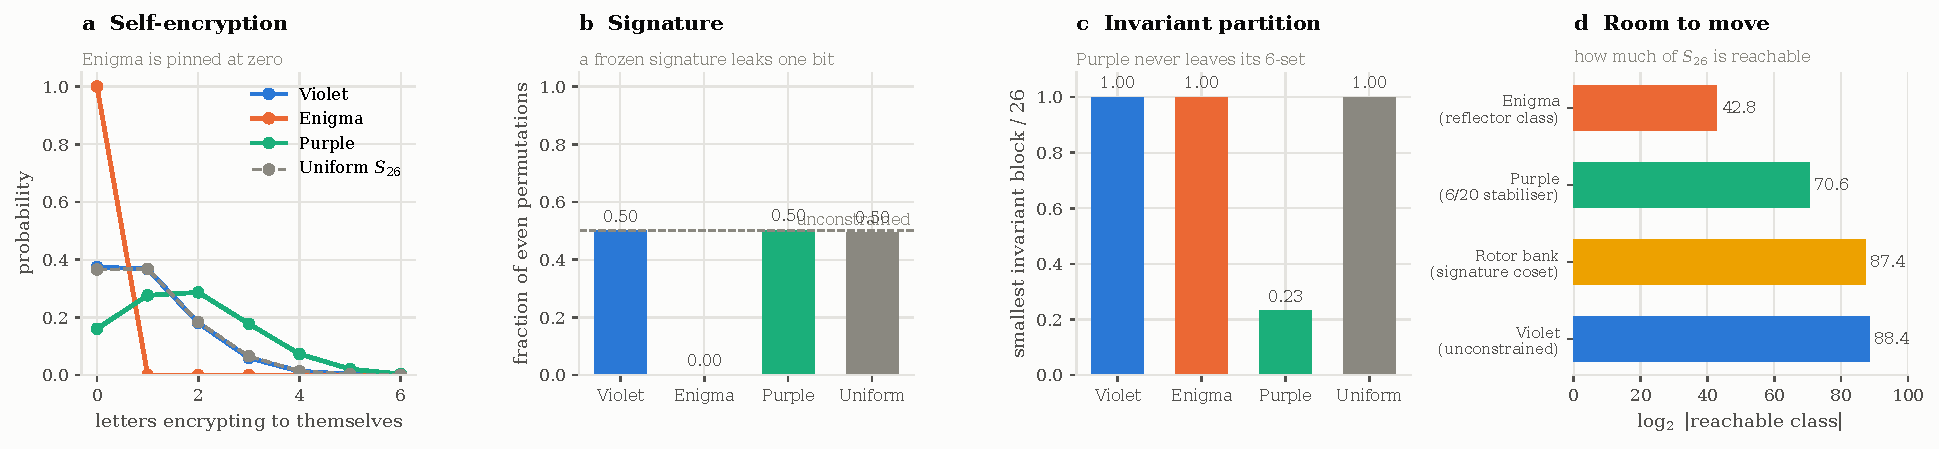
\includegraphics[width=\textwidth]{../figures/fig_invariants.pdf}
\caption{The three classical invariants, measured. (a) Enigma cannot encrypt a
letter to itself; Violet's fixed-point count is Poisson$(1)$, matching a uniform
draw from $S_{26}$. (b) A frozen signature is a free bit; the switch bank
unfreezes it. (c) An orbit computation recovers Purple's six-letter block from
ciphertext alone. (d) How much of $S_{26}$ each machine can reach before a key
is chosen.}
\label{fig:invariants}
\end{figure}

\section{The machine}\label{sec:violet}

\subsection{Data path}

Violet composes a rotor bank, a switch bank and a plugboard:
\begin{equation}\label{eq:datapath}
  E_t \;=\; \sigma\bigl(q^{(t)}\bigr)\,\circ\,\rho\bigl(p^{(t)}\bigr)\,\circ\,P,
  \qquad p^{(t)} \in \ZZ_{26}^{\,r},\ q^{(t)} \in \ZZ_{25}^{\,k}.
\end{equation}
There is no reflector, so $E_t$ is not an involution and $\Fix(E_t)$ is
generically nonempty; there is no alphabet split, so all $26$ letters traverse
every component. The \emph{inter-stage tap} is the wire between the two banks,
\begin{equation}\label{eq:tap}
  g_t \;=\; \rho\bigl(p^{(t)}\bigr)\bigl(P(x_t)\bigr) \;=\;
  \sigma\bigl(q^{(t)}\bigr)^{-1}(y_t),
\end{equation}
a physically existing conductor whose value the receiver can compute from the
ciphertext letter and its own state before it needs to step.

\subsection{Control path}

Two regimes are defined on the same data path.

\begin{definition}[Autonomous regime]
$p^{(t+1)} = \mathrm{odo}_{26}(p^{(t)})$ and $q^{(t+1)} = \mathrm{odo}_{25}(q^{(t)})$.
\end{definition}

\begin{definition}[Tap-driven regime]\label{def:closed}
The switch bank remains an autonomous odometer, $q^{(t+1)} =
\mathrm{odo}_{25}(q^{(t)})$. The rotor bank steps irregularly: rotor $0$ always
advances, and rotor $i \ge 1$ advances by $\mathrm{pin}_i(g_t) \in \{0,1\}$,
where $\mathrm{pin}_i : \ZZ_{26} \to \{0,1\}$ is a key-set ring of $26$ pins on
rotor $i$.
\end{definition}

The control rule is a Hagelin-style pin mechanism read by the tap conductor
rather than by a lug cage, and the two paradigms are coupled in the control path
rather than merely stacked in the data path: the switch bank sets the clock, the
rotor bank obeys it irregularly, and the letter being enciphered decides how.

\begin{proposition}[Correctness]\label{prop:correct}
For every build, every key, every regime and every message $x$, decryption
recovers $x$.
\end{proposition}

\begin{proof}
By induction on message length. At each step the receiver holds the same state
as the sender, computes $g_t = \sigma(q^{(t)})^{-1}(y_t)$ by
\eqref{eq:tap}, recovers $x_t = P^{-1}\rho(p^{(t)})^{-1}(g_t)$, and applies the
same stepping rule to the same $g_t$, so the states agree at $t+1$. The
statement and proof are formalised for an arbitrary stepping rule in
\lean{Machine.decrypt\_encrypt} (Section~\ref{sec:lean}).
\end{proof}

The proposition is stronger than it looks: it holds for \emph{any} stepping rule
whose argument is computable from the ciphertext and the current state. That is
the precise design freedom feedback buys, and it costs nothing in
synchronisation.

\subsection{Parameters}

We name two configurations.

\begin{center}
\small
\begin{tabular}{lrrrrrr}
\toprule
& rotors $r$ & chest & switches $k$ & plug pairs & $\log_2|\Om|$ & period \\
\midrule
Violet 8/8 (field)      & 8  & 12 & 8  & 10 & $74.8$  & $650^{8} = 3.19\times10^{22}$\\
Violet 14/14 (strategic)& 14 & 18 & 14 & 10 & $130.8$ & $650^{14} = 2.40\times10^{39}$\\
\bottomrule
\end{tabular}
\end{center}

\section{Periodicity}\label{sec:period}

\begin{theorem}[Exact period, autonomous regime]\label{thm:period}
In the autonomous regime the joint state is the pair of counters
$(v + t \bmod 26^{r},\ w + t \bmod 25^{k})$, and the state returns to its start
exactly at multiples of $26^{r}25^{k}$. The states at times $0,\dots,26^{r}25^{k}-1$
are pairwise distinct.
\end{theorem}

\begin{proof}
By Lemma~\ref{lem:odo} each bank is a counter, so the state at time $t$ is
$(v+t, w+t)$ in $\ZZ_{26^r}\times\ZZ_{25^k}$. It equals $(v,w)$ iff $26^{r}\mid t$
and $25^{k}\mid t$. Since $\gcd(26,25)=1$ we have $\gcd(26^{r},25^{k}) = 1$, so
the two divisibilities hold together iff $26^{r}25^{k}\mid t$. Distinctness
follows by applying this to $t'-t$.
\end{proof}

Theorem~\ref{thm:period} is the good news about coprimality and
Theorem~\ref{thm:transparency} will be the bad news about the same structure. It
is worth stating the bad news in its own right here:

\begin{corollary}[Open-loop transparency]\label{cor:transparent}
In the autonomous regime the state after $t$ letters depends on $t$ and the key
only. In particular two messages of equal length encrypted under one key
traverse identical state sequences, and a crib may be tested at position $t$
without knowledge of the preceding plaintext.
\end{corollary}

The tap-driven regime destroys Corollary~\ref{cor:transparent} by construction.
The concern this normally raises is that a message-dependent stepping rule
carries no period guarantee: nothing prevents an unlucky message from driving
the machine into a short cycle. Retaining one autonomous component answers the
concern completely.

\begin{theorem}[Period floor under arbitrary control]\label{thm:floor}
Let the state be $(p,q) \in \Pi \times \ZZ_{K}$ for an arbitrary set $\Pi$, and
let the trajectory be
\[
  p^{(t+1)} = F_t\bigl(p^{(t)}, q^{(t)}\bigr),\qquad q^{(t+1)} = q^{(t)} + 1,
\]
where $F_t$ is \emph{arbitrary} --- it may depend on the time, the plaintext, the
ciphertext, the pin rings, and the whole history. Then the states at times
$0,\dots,K-1$ are pairwise distinct. For Violet, $K = 25^{k}$, giving a floor of
$25^{14} > 2^{65}$ letters in the strategic configuration.
\end{theorem}

\begin{proof}
Project onto the second coordinate: $q^{(t)} = q^{(0)} + t$ in $\ZZ_K$. If
$t,t' < K$ and the states agree then $t \equiv t' \pmod K$, so $t = t'$.
\end{proof}

The proof is three lines and the design consequence is the paper's central one.
Feedback and a period guarantee are usually presented as a trade; they are not,
provided one component of the state remains autonomous and its modulus is the
guarantee. The bottleneck that made the classical machines analysable ---
a clock that ticks regardless of the message --- is retained exactly where it
produces a theorem and removed exactly where it produced the vulnerability.

\section{Security accounting}\label{sec:accounting}

\subsection{The transparency theorem}

Write the cascade as $E_t = C_t \circ P$, where $C_t = \sigma(q^{(t)})\rho(p^{(t)})$
is the moving composite and $P$ is static. An attacker who hypothesises a
trajectory $\widehat{C}$ forms the \emph{reduced stream}
$z_t = \widehat{C}_t^{-1}(y_t)$.

\begin{theorem}[Plugboard determination]\label{thm:plugdet}
If $y_t = C_t(P(x_t))$ for all $t$, then $P(x_t) = C_t^{-1}(y_t)$. Hence under
the correct trajectory hypothesis each known-plaintext position determines one
value of $P$ outright, and $P$ is recovered in time $O(L)$ once the trajectory
is known. If the crib exercises every letter, $P$ is unique.
\end{theorem}

\begin{proof}
Apply $C_t^{-1}$ to both sides. Uniqueness: two plugboards agreeing on a
surjective $x$ agree everywhere.
\end{proof}

\begin{corollary}[Repeated-letter test]\label{cor:repeat}
If $x_s = x_t$ then $C_s^{-1}(y_s) = C_t^{-1}(y_t)$, an equation in the
trajectory alone. A crib therefore yields plugboard-free consistency tests at a
rate governed by the letter-repetition density of the language.
\end{corollary}

Corollary~\ref{cor:repeat} is the structural analogue of Turing's loop test,
obtained here without a reflector and without a diagonal board: it is the
one-sided plugboard, not the reflector, that makes it available.

\begin{theorem}[Static-layer transparency]\label{thm:transparency}
Let $\mathrm{Co}_L(z) = \#\{(i,j): i<j<L,\ z_i = z_j\}$ be the coincidence count.
Then $\mathrm{Co}_L(P\circ x) = \mathrm{Co}_L(x)$ for every permutation $P$.
Consequently, under the correct trajectory hypothesis the coincidence count of
the reduced stream equals that of the plaintext, for every plugboard; the
statistic that identifies the trajectory is independent of $P$.
\end{theorem}

\begin{proof}
$P$ is injective, so $P(x_i) = P(x_j) \iff x_i = x_j$ and the two counted sets
are equal.
\end{proof}

\begin{corollary}[Effective key length]\label{cor:effective}
For a cascade with public wiring, known-plaintext key recovery costs
$\Theta(|\Om| L)$ where $\Om$ is the reachable state set, independently of the
plugboard's size. In particular the plugboard's $\log_2\binom{26}{2,\dots}
= 47.1$ bits contribute $0$ bits of work factor.
\end{corollary}

We stress what is and is not proved. Corollary~\ref{cor:effective} is an
\emph{upper} bound on security --- an attack achieving it is given in
Section~\ref{sec:attack}. We do not prove a matching lower bound; no attack
below $|\Om|$ is known for the autonomous cascade, and the gap is stated as open
in Section~\ref{sec:open}.

\begin{principle}[Key material must move]\label{rule:move}
Every bit of key must alter the state trajectory. Key material composed at the
boundary of a cascade is inert: it neither changes the trajectory nor perturbs
any relabelling-invariant statistic of the reduced stream.
\end{principle}

Design rule~\ref{rule:move} is what puts the pin rings in
Definition~\ref{def:closed}. Pins are not an ornament on the plugboard's model;
they are the plugboard's key material moved from the boundary, where
Theorem~\ref{thm:transparency} makes it worthless, into the stepping law, where
it is not.

\begin{figure}[t]
\centering
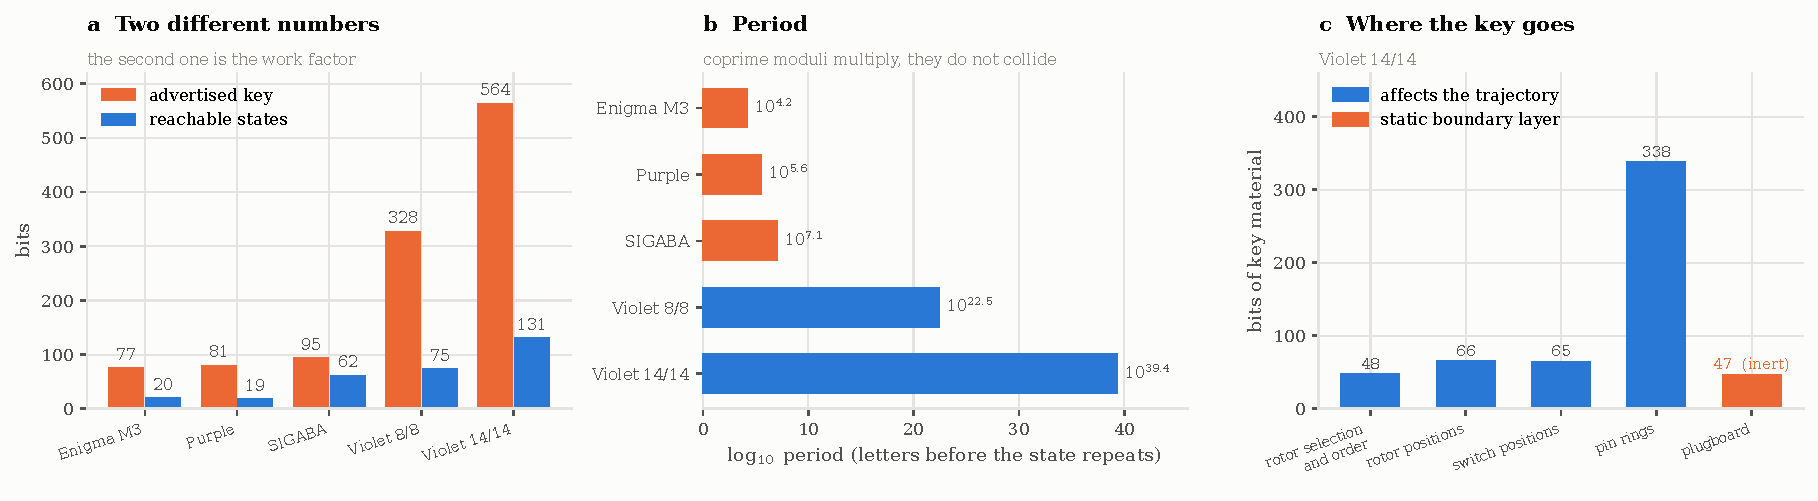
\includegraphics[width=\textwidth]{../figures/fig_security.pdf}
\caption{Security accounting. (a) Advertised key length against the size of the
reachable state set, which is what the attack of Section~\ref{sec:attack}
enumerates. (b) Period, on a log scale; coprime moduli multiply.
(c) Where the key of a Violet 14/14 goes: everything that moves the trajectory
counts, the boundary layer does not.}
\label{fig:security}
\end{figure}

\subsection{How much hardware a security level costs}

Corollary~\ref{cor:effective} converts directly into a specification. Ignoring
pin rings, whose contribution we bound rather than determine, a cascade attains
$s$ bits of proven-floor security iff
\begin{equation}\label{eq:sizing}
  r\log_2 26 + k\log_2 25 \;\ge\; s .
\end{equation}
With $r = k$ this is $r \ge s/9.31$: $s = 128$ needs $r = k = 14$. The
corresponding unicity distance, at an English redundancy of
$\log_2 26 - 1.5 = 3.20$ bits per letter, is $130.8/3.20 = 40.9$ letters ---
about eight words of crib is all the information the cipher can hide behind.

\section{Key recovery}\label{sec:attack}

\subsection{The algorithm}

\begin{quote}\small
\textbf{Input:} public build; crib $x_{0..L-1}$ with ciphertext $y_{0..L-1}$.\\
\textbf{For} each state hypothesis $(c,d) \in \ZZ_{26^{r}}\times\ZZ_{25^{k}}$:
\begin{enumerate}[nosep,leftmargin=2em]
\item For $t = 0,1,\dots$: set $z_t = \rho_{c+t}^{-1}\bigl(\sigma_{d+t}^{-1}(y_t)\bigr)$.
\item Maintain the partial map $x_t \mapsto z_t$; reject as soon as it fails to
extend to an involution with at most $\pi$ transpositions and at most
$26-2\pi$ fixed points.
\end{enumerate}
\textbf{Output:} the surviving $(c,d)$, and $P$ read off by Theorem~\ref{thm:plugdet}.
\end{quote}

The plugboard is never enumerated: it appears only as a consistency predicate,
and the predicate is checked incrementally, so a wrong hypothesis is killed
after a constant number of letters in expectation.

\begin{theorem}[Attack complexity]\label{thm:attackcost}
The algorithm terminates in time $O(|\Om|\cdot \bar{L})$ where $\bar{L} = O(1)$
is the expected rejection depth, and uses $O(26^{r} + 25^{k})$ memory for the
stage tables. It outputs the true key, and the expected number of spurious
survivors after $L$ crib letters is $|\Om| \cdot \Pr[\text{random map passes}]$,
which falls below $1$ at $L \approx \log_2|\Om| / D_{\mathrm{filt}}$, where
$D_{\mathrm{filt}} \le D$ is the number of bits the consistency test removes per
letter and $D$ is the redundancy of the plaintext language.
\end{theorem}

\begin{proof}
Correctness is Theorem~\ref{thm:plugdet}: the true hypothesis yields
$z_t = P(x_t)$, which is consistent by construction. The cost statement follows
because each hypothesis is tested by table lookups, and the survival probability
of a wrong hypothesis decays geometrically in $t$, so the expected work per
hypothesis is constant. The survivor estimate is the standard unicity-distance
argument applied with key entropy $\log_2|\Om|$.
\end{proof}

\subsection{Measurements}

We instantiated the attack in C with OpenMP and ran it to completion on seven
scaled builds, from $|\Om| = 4.2\times10^{5}$ to $|\Om| = 1.8\times10^{11}$, on
36~cores. In every run exactly one hypothesis survived, and it was the true one.
Figure~\ref{fig:attack}a shows wall-clock time against $|\Om|$; the fitted
exponent on the runs large enough for table construction to be negligible is
$1.01$, at a sustained $2.85\times10^{8}$ hypotheses per second, confirming the
linear scaling of Theorem~\ref{thm:attackcost}. Figure~\ref{fig:attack}b shows
the survivor count against crib length. The plugboard-consistency filter removes
$2.68$ bits per letter --- below the $3.20$ bits of English redundancy, as it
must be, since the filter uses no language model at all --- and a unique key
emerges after $10$ letters at $18.7$ key bits and $18$ letters at $37.4$. The
observed unicity distance therefore tracks $\log_2|\Om|/2.68$ rather than the
information-theoretic $\log_2|\Om|/3.20$; a filter that also scored English
statistics would close the difference.

Extrapolating the measured throughput to the canonical builds, Violet 8/8 falls
at $2^{74.8}$ and Violet 14/14 at $2^{130.8}$ state hypotheses --- the first
within reach of a determined adversary with modern hardware, the second not.
The distance between the two is eight bits of rotor and eight of switch, and
nothing else in the key matters to it.

\begin{figure}[t]
\centering
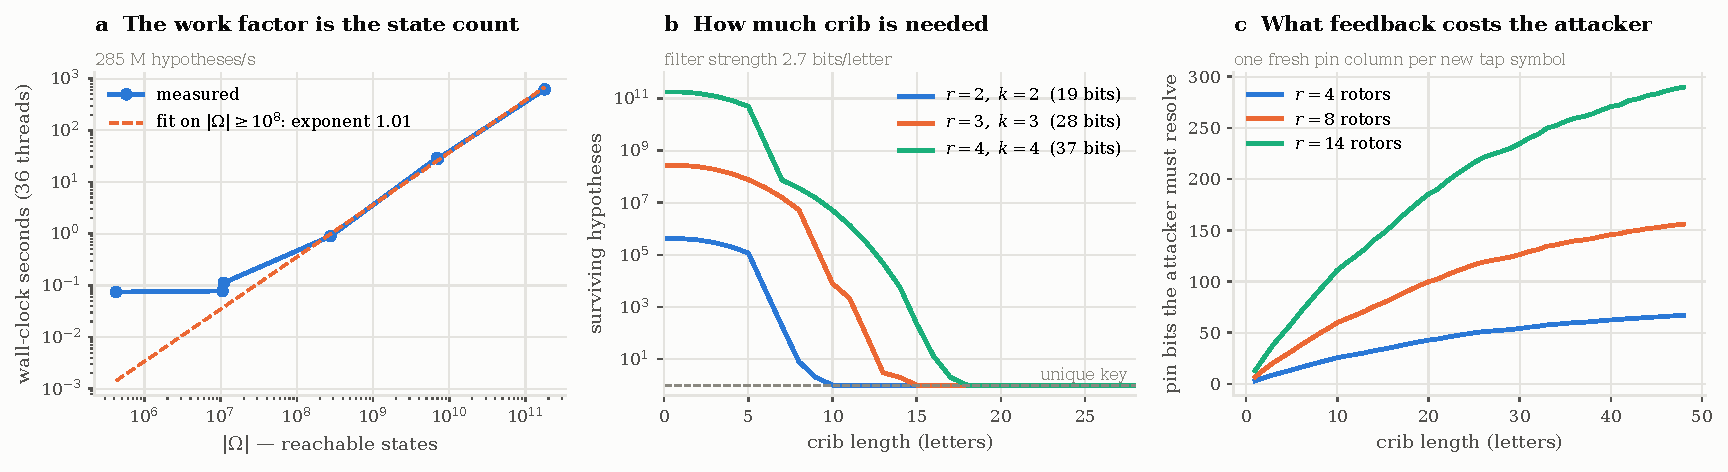
\includegraphics[width=\textwidth]{../figures/fig_attack.pdf}
\caption{Key recovery, measured. (a) Exhaustive trajectory search over seven
scaled builds; the fitted exponent confirms cost $\Theta(|\Om|)$. (b) Surviving
hypotheses against crib length; a unique key emerges at the unicity distance,
with the plugboard never enumerated. (c) Under tap-driven stepping the attacker
must additionally resolve one column of the pin matrix per distinct tap symbol.}
\label{fig:attack}
\end{figure}

\subsection{The attack against the tap-driven regime}

The algorithm above does not apply to Definition~\ref{def:closed}, because step
1 presumes $p^{(t)} = c + t$. An attacker must instead guess the pin columns as
they are first used. Each newly seen tap value exposes one fresh column of the
$(r{-}1)\times 26$ pin matrix, so after $L$ crib letters the pin entropy in play
is $(r-1)\cdot d(L)$ bits, where $d(L)$ is the number of distinct tap symbols
observed; $d$ saturates at $26$. Figure~\ref{fig:attack}c plots the measured
$(r-1)d(L)$. Against this the crib supplies about $\log_2 26 = 4.7$ bits of
constraint per letter, so a branch-and-prune search is a race between a
branching factor of $2^{r-1}$ on fresh symbols and a pruning factor of $1/26$
per letter. For $r \le 5$ pruning wins and the search is feasible; for
$r = 14$ the branching factor is $2^{13}$ against a pruning factor of $2^{-4.7}$
and the tree grows. We do not claim a bound here; determining the true
complexity of pin recovery is the main open problem left by this work.

\section{What feedback buys}\label{sec:feedback}

\begin{theorem}[Error propagation]\label{thm:avalanche}
Model $E_t$ at distinct states as independent uniform draws from
$\Sym(\mathcal{A})$. In the tap-driven regime, if two messages first differ at
position $i$, then for every $j > i$ the ciphertexts differ at $j$ with
probability $1 - 1/26$, up to a resynchronisation term bounded by $j/|\Om|$. In
the autonomous regime the probability is $0$ for all $j > i$.
\end{theorem}

\begin{proof}
Autonomous: the states agree at every $j$, so $y_j$ depends only on $x_j$.
Tap-driven: at position $i$ the taps differ, so the rotor increments differ with
probability $1 - 2^{-(r-1)}$ over the pin ring, and once the states differ the
two permutations are independent draws, giving agreement probability $1/26$ per
position. Resynchronisation requires the two rotor states to coincide again
while the switch states already agree, an event of probability at most
$1/26^{r}$ per step by Theorem~\ref{thm:floor}; union bound over $j$ steps.
\end{proof}

Measured over $60$ keys and $200$ positions the tap-driven change rate is
$0.9624$ against the predicted $25/26 = 0.9615$, and the autonomous rate is
exactly $0$ (Figure~\ref{fig:diffusion}a,c). For the strategic configuration the
resynchronisation bound is $1.6\times10^{-20}$ per step.

\begin{theorem}[Destruction of depth]\label{thm:depth}
In the autonomous regime two messages of equal length under one key induce
identical state sequences. In the tap-driven regime the sequences separate at
the first position where the taps differ and, up to the resynchronisation term
of Theorem~\ref{thm:avalanche}, do not rejoin.
\end{theorem}

Measured over $40$ key/message pairs, autonomous trajectories agree at every one
of $120$ positions and tap-driven trajectories agree at none after position four
(Figure~\ref{fig:diffusion}b). Depth is the resource that Banburismus, the
Bombe's menu construction and Purple's reconstruction all consumed; the
tap-driven regime does not supply it.

The cost is the standard cost of self-synchronising feedback: a garbled
ciphertext letter corrupts the following letters until the state
resynchronises, which for the tap-driven rule it does not do. Operationally,
messages must be short enough that a transmission error is cheaper to
retransmit than to reconstruct --- the same discipline that applies to any
chained cipher, and the reason the field configuration exists.

\begin{figure}[t]
\centering
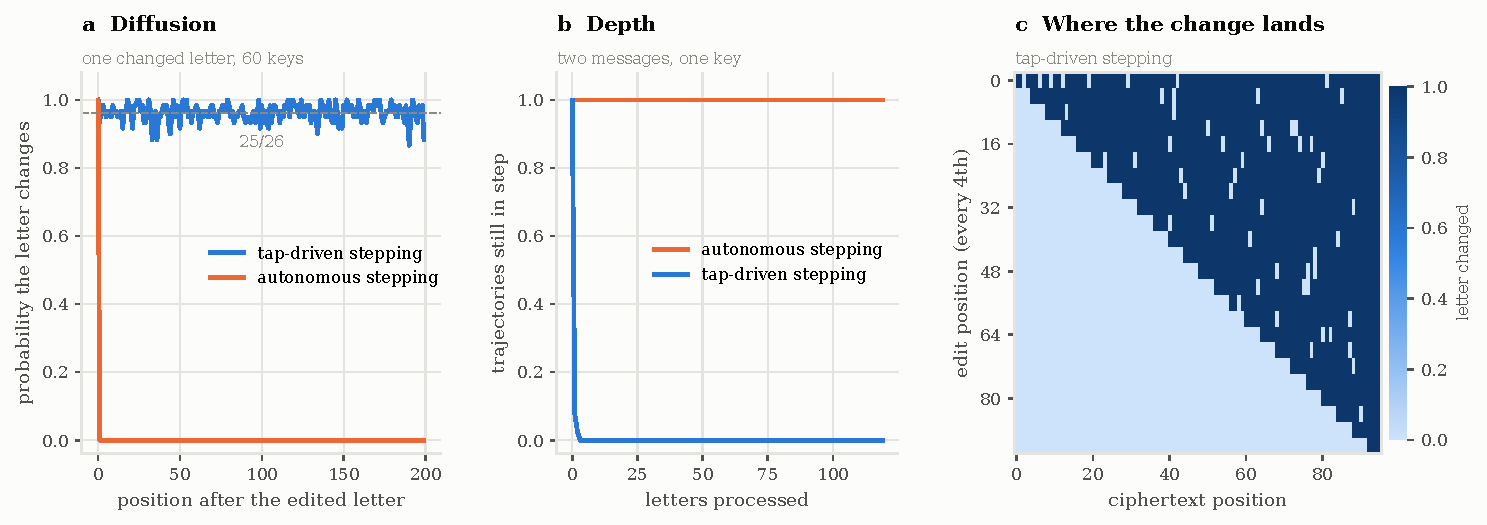
\includegraphics[width=\textwidth]{../figures/fig_diffusion.pdf}
\caption{Feedback in the control path. (a) A single changed letter alters
$96.2\%$ of all later ciphertext under tap-driven stepping and none of it under
autonomous stepping. (b) Two messages under one key: autonomous trajectories
stay locked, tap-driven ones separate within four letters. (c) The same edit
applied at $24$ positions.}
\label{fig:diffusion}
\end{figure}

\section{Statistical behaviour}\label{sec:stats}

Over a $20\,000$-letter English message the ciphertext $\chi^{2}$ against
uniform falls from $12\,472$ to $20.3$ on $25$ degrees of freedom (critical
value $37.65$ at $\alpha = 0.05$), and the index of coincidence falls from
$0.0624$ to $0.03845$ against the uniform value $1/26 = 0.038462$
(Figure~\ref{fig:statistics}a,b). Both regimes give the same answer to three
digits, which is the expected result: flattening is a property of the data path,
and the two regimes share it.

The third panel is the one that matters. For $40$ independent plugboards we
computed the coincidence index of the reduced stream under the correct
trajectory and under $240$ wrong ones. The correct trajectory returns the
plaintext value $0.0653$; wrong trajectories return $0.0384$; the separation is
$61.4$ standard deviations and does not vary with the plugboard, exactly as
Theorem~\ref{thm:transparency} requires. An attacker sorting state hypotheses by
this statistic never needs to consider $P$ at all.

\begin{figure}[t]
\centering
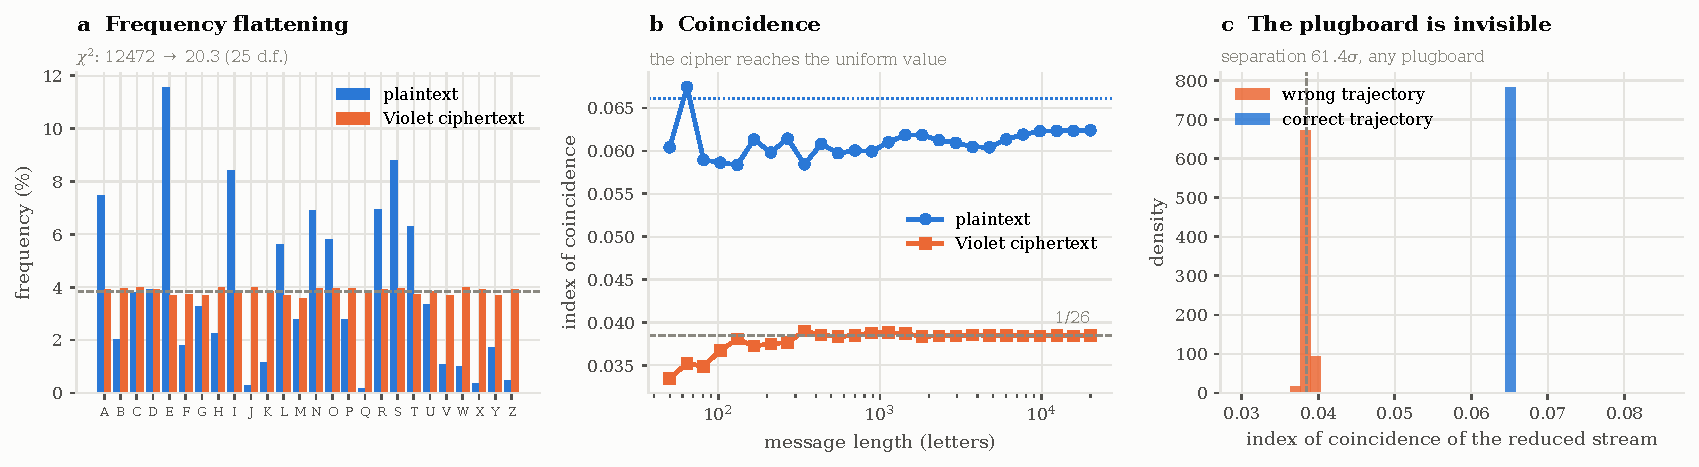
\includegraphics[width=\textwidth]{../figures/fig_statistics.pdf}
\caption{Ciphertext statistics. (a) English letter frequencies against Violet
ciphertext. (b) Index of coincidence against message length. (c) The statistic
that identifies a trajectory, computed under $40$ different plugboards: the
separation is $61.4\sigma$ and the plugboard is invisible to it.}
\label{fig:statistics}
\end{figure}

\section{Mechanical realisability}\label{sec:hardware}

Every component is period technology. The rotor bank is a stack of wired discs
with a Geneva-type advance, as in the Enigma and the SIGABA; a $14$-rotor stack
is heavier than the SIGABA's $15$ but of the same order. The switch bank is
$14$ Strowger selectors, each a $25$-level uniselector of the kind installed by
the hundred in a telephone exchange. The plugboard is a patch panel. The pin
rings are Hagelin's mechanism: a $26$-pin ring per rotor, each pin set left or
right by hand, read by a follower.

The only element without an exact wartime precedent is the tap reader: a decoder
that converts the $26$-way inter-stage conductor into the $r-1$ step/no-step
signals for rotors $1..r-1$. It is a $26$-input, $(r{-}1)$-output diode or relay
matrix whose $26 \times (r{-}1)$ crosspoints are the pin settings, energised
from the conductor that is already carrying the signal. In 1943 terms this is a
relay tree of the sort used for translator circuits in exchanges, and it adds
one relay step to the per-character cycle. The key-setting burden is $r$ rotor
positions, $k$ switch positions, $\pi$ plug pairs and $(r{-}1)\times 26$ pins;
the pins are a long-period key, changed weekly, exactly as Hagelin's were.

\section{Formal development}\label{sec:lean}

The structural results are machine-checked in Lean~4 against \emph{mathlib}: a
development of $45$ theorems across five files, compiling with no incomplete
proofs and no axioms beyond \emph{mathlib}'s.

\begin{center}
\small
\begin{tabular}{llp{6.1cm}}
\toprule
Result & Lean name & Content \\
\midrule
Prop.~\ref{prop:correct} & \lean{Machine.decrypt\_encrypt} & Decryption inverts encryption for an \emph{arbitrary} stepping rule \\
--- & \lean{Machine.encrypt\_injective} & The map is a cipher \\
Cor.~\ref{cor:transparent} & \lean{Machine.runState\_autonomous} & Autonomous state is a function of message \emph{length} \\
--- & \lean{Machine.autonomous\_depth} & Equal-length messages share a trajectory \\
Thm.~\ref{thm:period} & \lean{jointStep\_fixed\_iff} & Return time is exactly $\mathrm{lcm}$, via coprimality \\
--- & \lean{jointStep\_injOn} & No repeat inside one period \\
Thm.~\ref{thm:floor} & \lean{closed\_loop\_period\_floor} & Floor $K$ under an arbitrary rotor rule \\
Thm.~\ref{thm:reflector} & \lean{IsReflector.conj} & Conjugates of a reflector are reflectors \\
--- & \lean{reflector\_no\_self\_encryption} & $E(x)\neq x$ \\
Thm.~\ref{thm:signature} & \lean{sign\_rotorStage} & $\sgn\rho(p) = \prod_i \sgn W_i$, for all $p$ \\
Thm.~\ref{thm:partition} & \lean{blockStabilizer} & Block-respecting permutations form a subgroup \\
Thm.~\ref{thm:plugdet} & \lean{plug\_determined}, \lean{plug\_unique} & Plugboard computed, and unique \\
Cor.~\ref{cor:repeat} & \lean{repeat\_letter\_test} & Plugboard-free equations from repeats \\
Thm.~\ref{thm:transparency} & \lean{coincidences\_reduce\_eq} & Coincidence count independent of $P$ \\
Def.~\ref{def:invfree} & \lean{InvariantFree} & The three escape conditions and their consequences \\
\bottomrule
\end{tabular}
\end{center}

Two choices in the formalisation are worth noting. First,
\lean{Machine.decrypt\_encrypt} is stated for a machine whose stepping rule
consumes an arbitrary symbol computable by the receiver, so a single proof
covers both regimes and any future rule of the same shape. Second,
\lean{closed\_loop\_period\_floor} quantifies over an arbitrary time-dependent
rotor rule $F$, which is the strongest form of the statement: it grants the
adversary complete control of the rotor bank and still forbids a repeat.

\section{Open problems}\label{sec:open}

\begin{enumerate}[leftmargin=1.4em]
\item \textbf{A lower bound for the autonomous cascade.} We prove security is at
most $\log_2|\Om|$ and know no attack below it. Is $\Om$-enumeration optimal, or
does the coprime structure admit a meet-in-the-middle below $|\Om|$? The
differential at period offsets is suggestive: $E_{t+25^{k}}^{-1}E_t$ eliminates
the switch bank and the plugboard simultaneously.
\item \textbf{The complexity of pin recovery.} Section~\ref{sec:attack}
identifies a branch-and-prune search with branching $2^{r-1}$ on fresh tap
symbols against $\log_2 26$ bits of constraint per letter. The threshold in $r$
at which pruning stops winning is not determined here.
\item \textbf{Optimal control couplings.} Definition~\ref{def:closed} taps the
inter-stage wire. Other taps --- the switch-bank output, a second rotor
sub-bank, a SIGABA-style index layer --- give different trade-offs between
diffusion rate and pin entropy. Which coupling maximises the proven floor per
unit of hardware is open.
\item \textbf{Formalising the attack.} The transparency theorems are verified;
the complexity statement of Theorem~\ref{thm:attackcost} is not, because a cost
model for the search would have to be formalised first.
\end{enumerate}

\section{Related work}\label{sec:related}

Rejewski's recovery of the Enigma wiring from permutation cycle structure
\cite{rejewski1980} and Turing's crib-based method \cite{turing1940} are the
origin of the analysis in Section~\ref{sec:attack}; the repeated-letter test of
Corollary~\ref{cor:repeat} plays the role Turing's loops play, and needs no
reflector. Deavours and Kruh \cite{deavours1985} and Bauer \cite{bauer2013} give
the machine descriptions we model. The recovery of the Type~B machine is
described by Rowlett \cite{rowlett1998} and analysed by Freeman
\emph{et al.}~\cite{freeman2003}; our Theorem~\ref{thm:partition} states the
structural fact their reconstruction exploited. Modern computational
cryptanalysis of the Enigma \cite{gillogly1995,sullivan2005,ostwald2017}
confirms empirically what Theorem~\ref{thm:reflector} states structurally: the
work factor is set by the rotor state count and the plugboard is recovered
afterwards, not searched. The design principle of Section~\ref{sec:accounting}
--- that key material must move the state --- is the electromechanical form of
Kerckhoffs' second requirement \cite{kerckhoffs1883}, sharpened from ``the key
must be changeable'' to ``the key must be dynamical''. Shannon's unicity
distance \cite{shannon1949} supplies the crib-length prediction we verify.
Irregular, key-controlled stepping is Hagelin's contribution
\cite{hagelin1994} and, in a different form, the SIGABA's
\cite{savard1999,stamp2007}; what is new here is retaining an autonomous
sub-clock \emph{as the carrier of the period proof} while the rest of the state
is message-driven.

\section{Conclusion}

The lesson of the two paradigms is not that reflectors and split alphabets are
bad ideas. It is that a machine's security is the size of the set of states its
messages can drive it through, and that everything else --- plugboards, wiring
chests, patch panels --- is bookkeeping unless it moves that set. The invariant
taxonomy explains what the classical attacks actually consumed; the transparency
theorem explains why composing the two paradigms does not help; the period-floor
theorem shows that the fix does not cost the guarantee it appears to.

Coprimality does the work in both directions. It multiplies the periods of the
two banks, and it makes one of them a clock that no message can perturb. A
design that keeps that clock and hands the rest of the state to the message gets
a proof and a diffusion rate at the same time.

\begin{thebibliography}{99}
\small
\bibitem{bauer2013} F.~L. Bauer. \emph{Decrypted Secrets: Methods and Maxims of Cryptology}. 4th ed., Springer, 2007.
\bibitem{deavours1985} C.~A. Deavours and L.~Kruh. \emph{Machine Cryptography and Modern Cryptanalysis}. Artech House, 1985.
\bibitem{freeman2003} W.~Freeman, G.~Sullivan, and F.~Weierud. Purple revealed: simulation and computer-aided cryptanalysis of Angooki Taipu B. \emph{Cryptologia}, 27(1):1--43, 2003.
\bibitem{gillogly1995} J.~J. Gillogly. Ciphertext-only cryptanalysis of Enigma. \emph{Cryptologia}, 19(4):405--413, 1995.
\bibitem{hagelin1994} B.~Hagelin. The story of the Hagelin cryptos. \emph{Cryptologia}, 18(3):204--242, 1994.
\bibitem{kerckhoffs1883} A.~Kerckhoffs. La cryptographie militaire. \emph{Journal des Sciences Militaires}, IX:5--38, 1883.
\bibitem{ostwald2017} O.~Ostwald and F.~Weierud. Modern breaking of Enigma ciphertexts. \emph{Cryptologia}, 41(5):395--421, 2017.
\bibitem{rejewski1980} M.~Rejewski. An application of the theory of permutations in breaking the Enigma cipher. \emph{Applicationes Mathematicae}, 16(4):543--559, 1980.
\bibitem{rowlett1998} F.~B. Rowlett. \emph{The Story of Magic: Memoirs of an American Cryptologic Pioneer}. Aegean Park Press, 1998.
\bibitem{savard1999} J.~J.~G. Savard and R.~S. Pekelney. The ECM Mark II: design, history and cryptology. \emph{Cryptologia}, 23(3):211--228, 1999.
\bibitem{shannon1949} C.~E. Shannon. Communication theory of secrecy systems. \emph{Bell System Technical Journal}, 28(4):656--715, 1949.
\bibitem{stamp2007} M.~Stamp and R.~M. Low. \emph{Applied Cryptanalysis: Breaking Ciphers in the Real World}. Wiley, 2007.
\bibitem{sullivan2005} G.~Sullivan and F.~Weierud. Breaking German Army ciphers. \emph{Cryptologia}, 29(3):193--232, 2005.
\bibitem{turing1940} A.~M. Turing. \emph{Treatise on the Enigma} (``Prof's Book''). GC\&CS, c.~1940; released by the National Archives, 1996.
\bibitem{mathlib2020} The mathlib Community. The Lean mathematical library. In \emph{CPP 2020}, pages 367--381. ACM, 2020.
\end{thebibliography}

\end{document}
